\documentclass{article}

\usepackage{arxiv}

\usepackage[utf8]{inputenc}
\usepackage[T1]{fontenc}
\usepackage{hyperref}
\hypersetup{
  colorlinks,
  linkcolor={red!50!black},
  citecolor={blue!50!black},
  urlcolor={blue!80!black}
}
\usepackage{url}
\usepackage{booktabs}
\usepackage{amsmath,amssymb,amsfonts}
\usepackage{microtype}
\usepackage{graphicx}
\usepackage{siunitx}

\usepackage[numbers,square,comma,sort&compress]{natbib}

\graphicspath{{./images/}{./}}

% ------------------------------------------------------------------
% Title and author
% ------------------------------------------------------------------
\title{Paper Title}

\author{
  Jason Jain, Dr. Jesse Rodriguez \\
  Oregon State University \\
  Coupled Systems Laboratory
}

\begin{document}
\maketitle

\begin{abstract}
A Tokamak is a torus-shaped nuclear fusion reactor design that uses magnetic fields to confine fusion fuel in the form of plasma. A single plasma experiement in a Tokamak is called a "shot", and can often experience disruption events that cause a current drop to zero. The existence of a computationally inexpensive model for classifying shots as disruptive/not-disruptive, as well as identifying the time of disruption, can assist the scientific community in conducting future experiements. We train a CNN (Convolutional Neural Network) on current time series data from 40,000 shots from the DIII-D Tokamak, and achieve a recall of 99\% and precision of 91\% on boolean disruption/not-disruption predictions. We additionally develop a convolutional heuristic that accurately identifies time of disruption with a standard deviation $\sigma=\qty{8.7}{\milli\sec}$.


\end{abstract}


% ==================================================================
\section{Introduction}
\label{sec:intro}

State the problem, motivation, and contributions.

% ==================================================================
\section{Methods}
\label{sec:methods}

Describe data, models, training, and evaluation.



\begin{figure}[t]
  \centering
  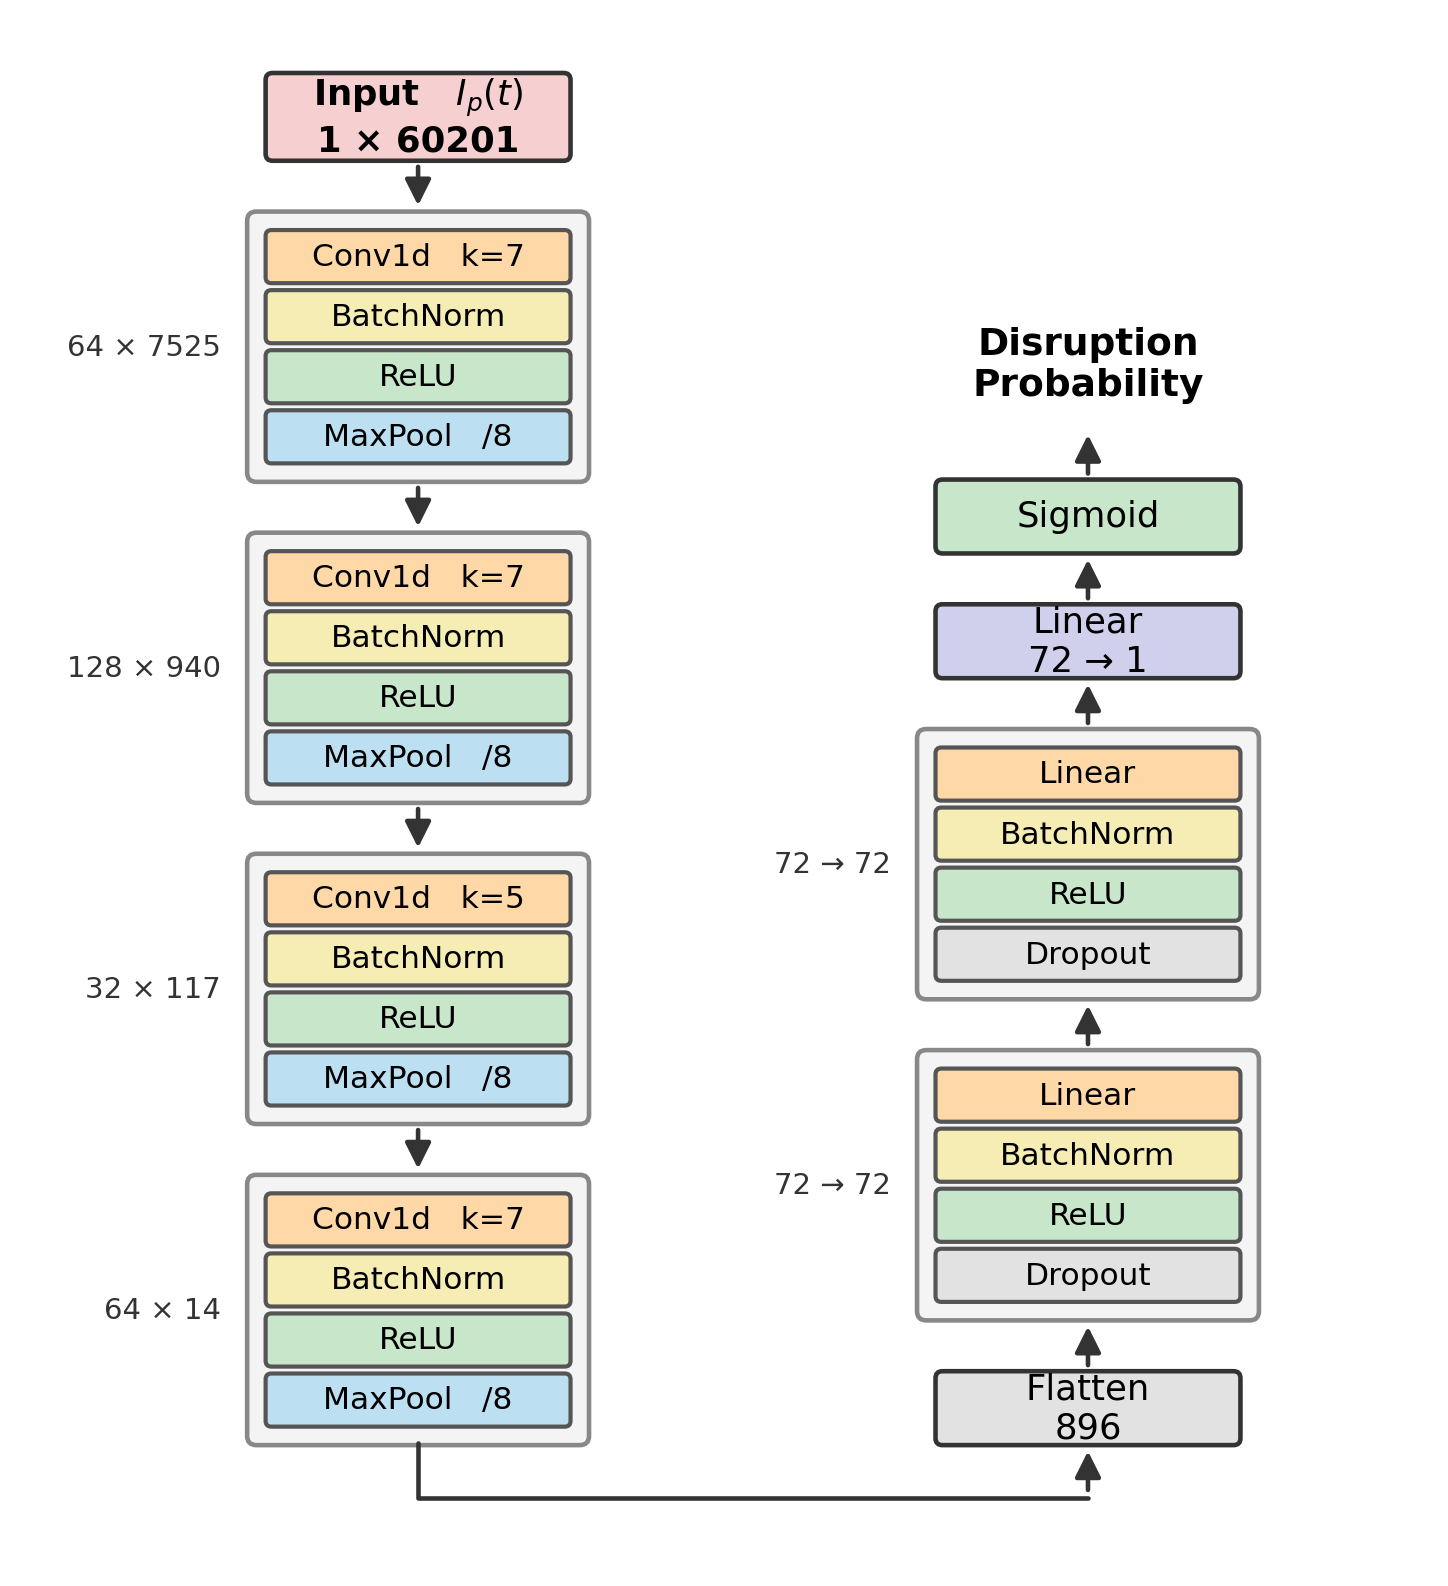
\includegraphics[width=0.8\linewidth]{best_model/model_diagram.png}
  \caption{Figure caption.}
  \label{fig:model_diagram}
\end{figure}


% ==================================================================
\section{Results}
\label{sec:results}

Report quantitative and qualitative findings. Reference figures and tables as needed.

\begin{figure}[t]
  \centering
  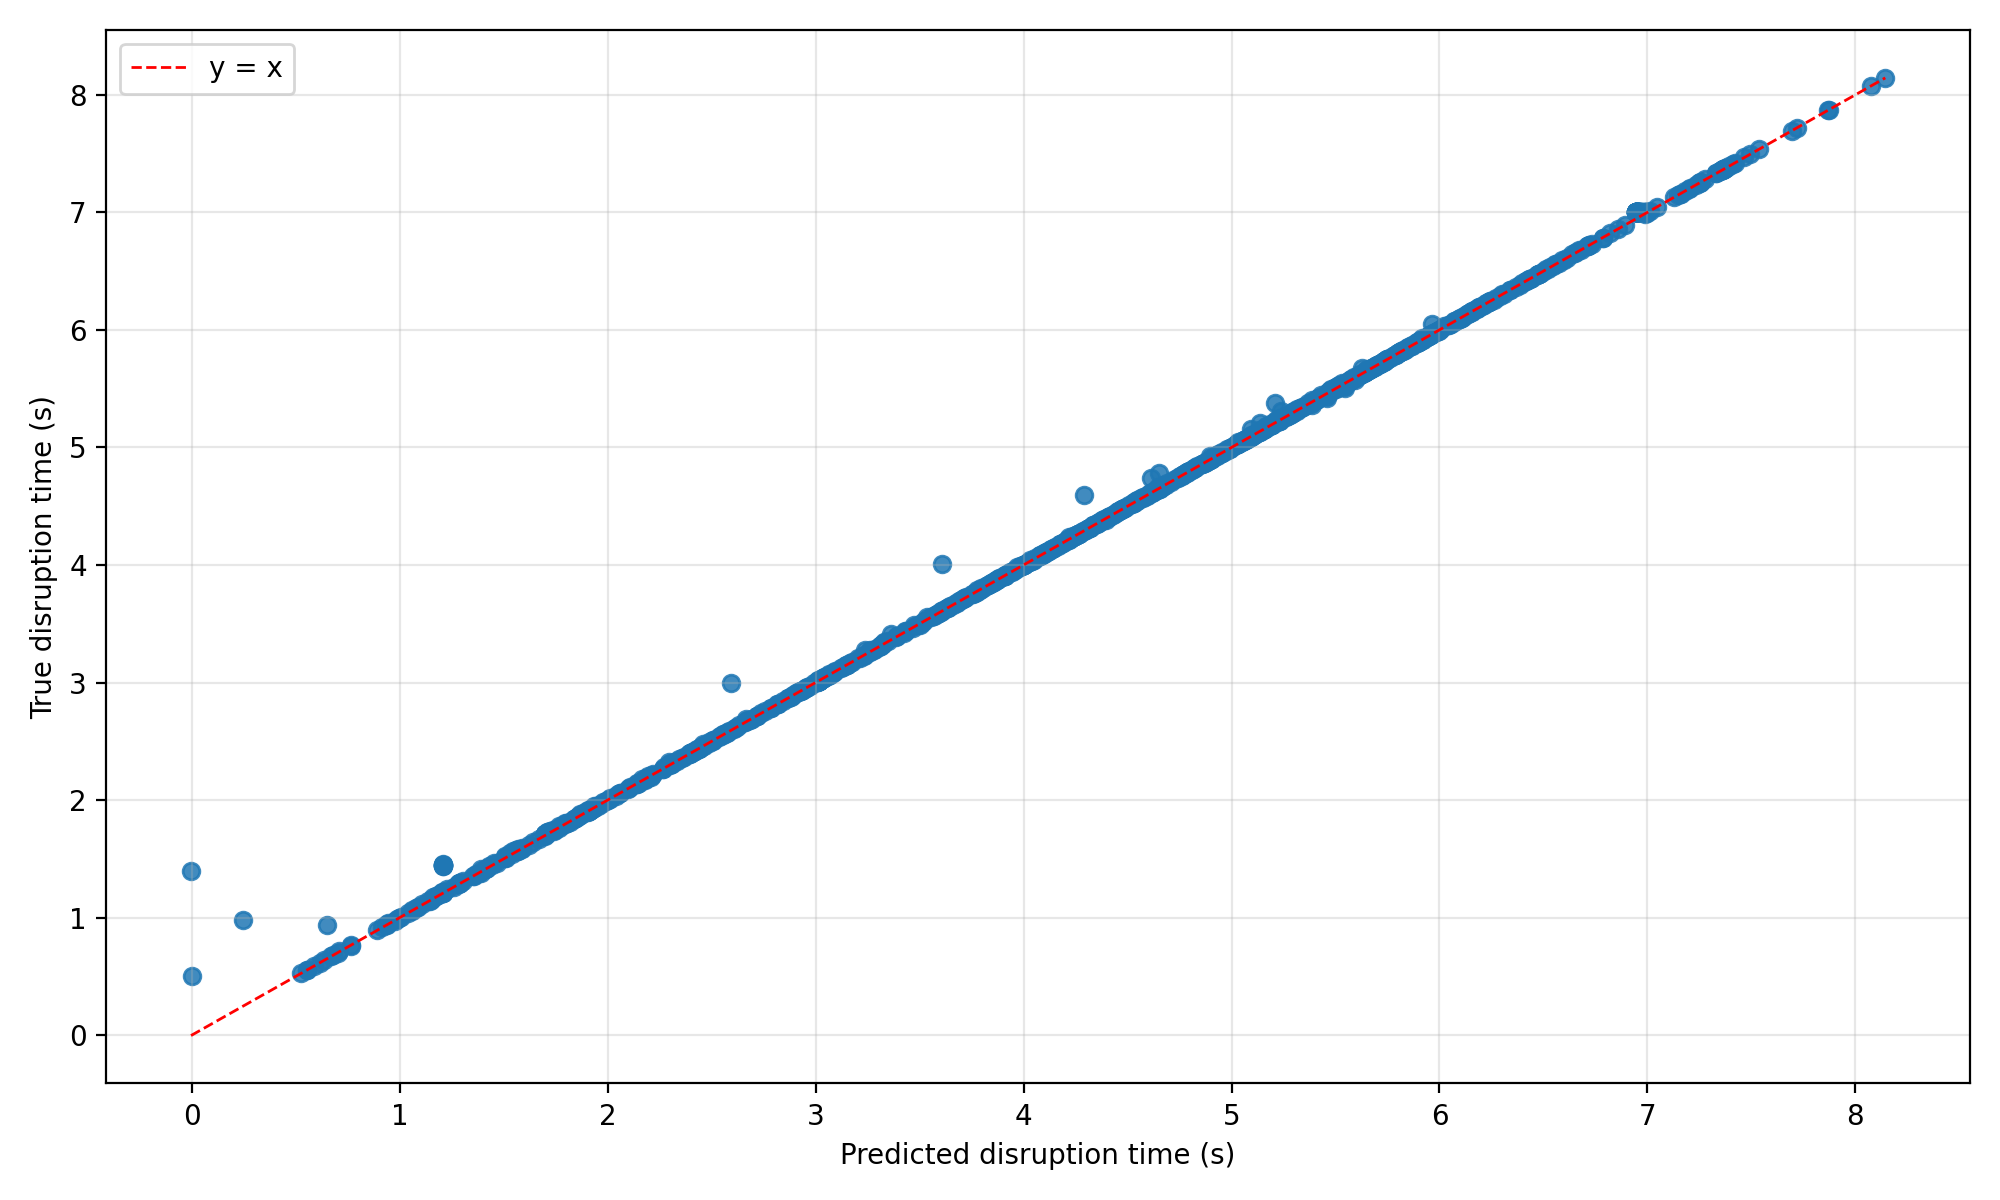
\includegraphics[width=0.8\linewidth]{best_model/predictions_scatter.png}
  \caption{Figure caption.}
  \label{fig:predictions_scatter}
\end{figure}

\begin{figure}[t]
  \centering
  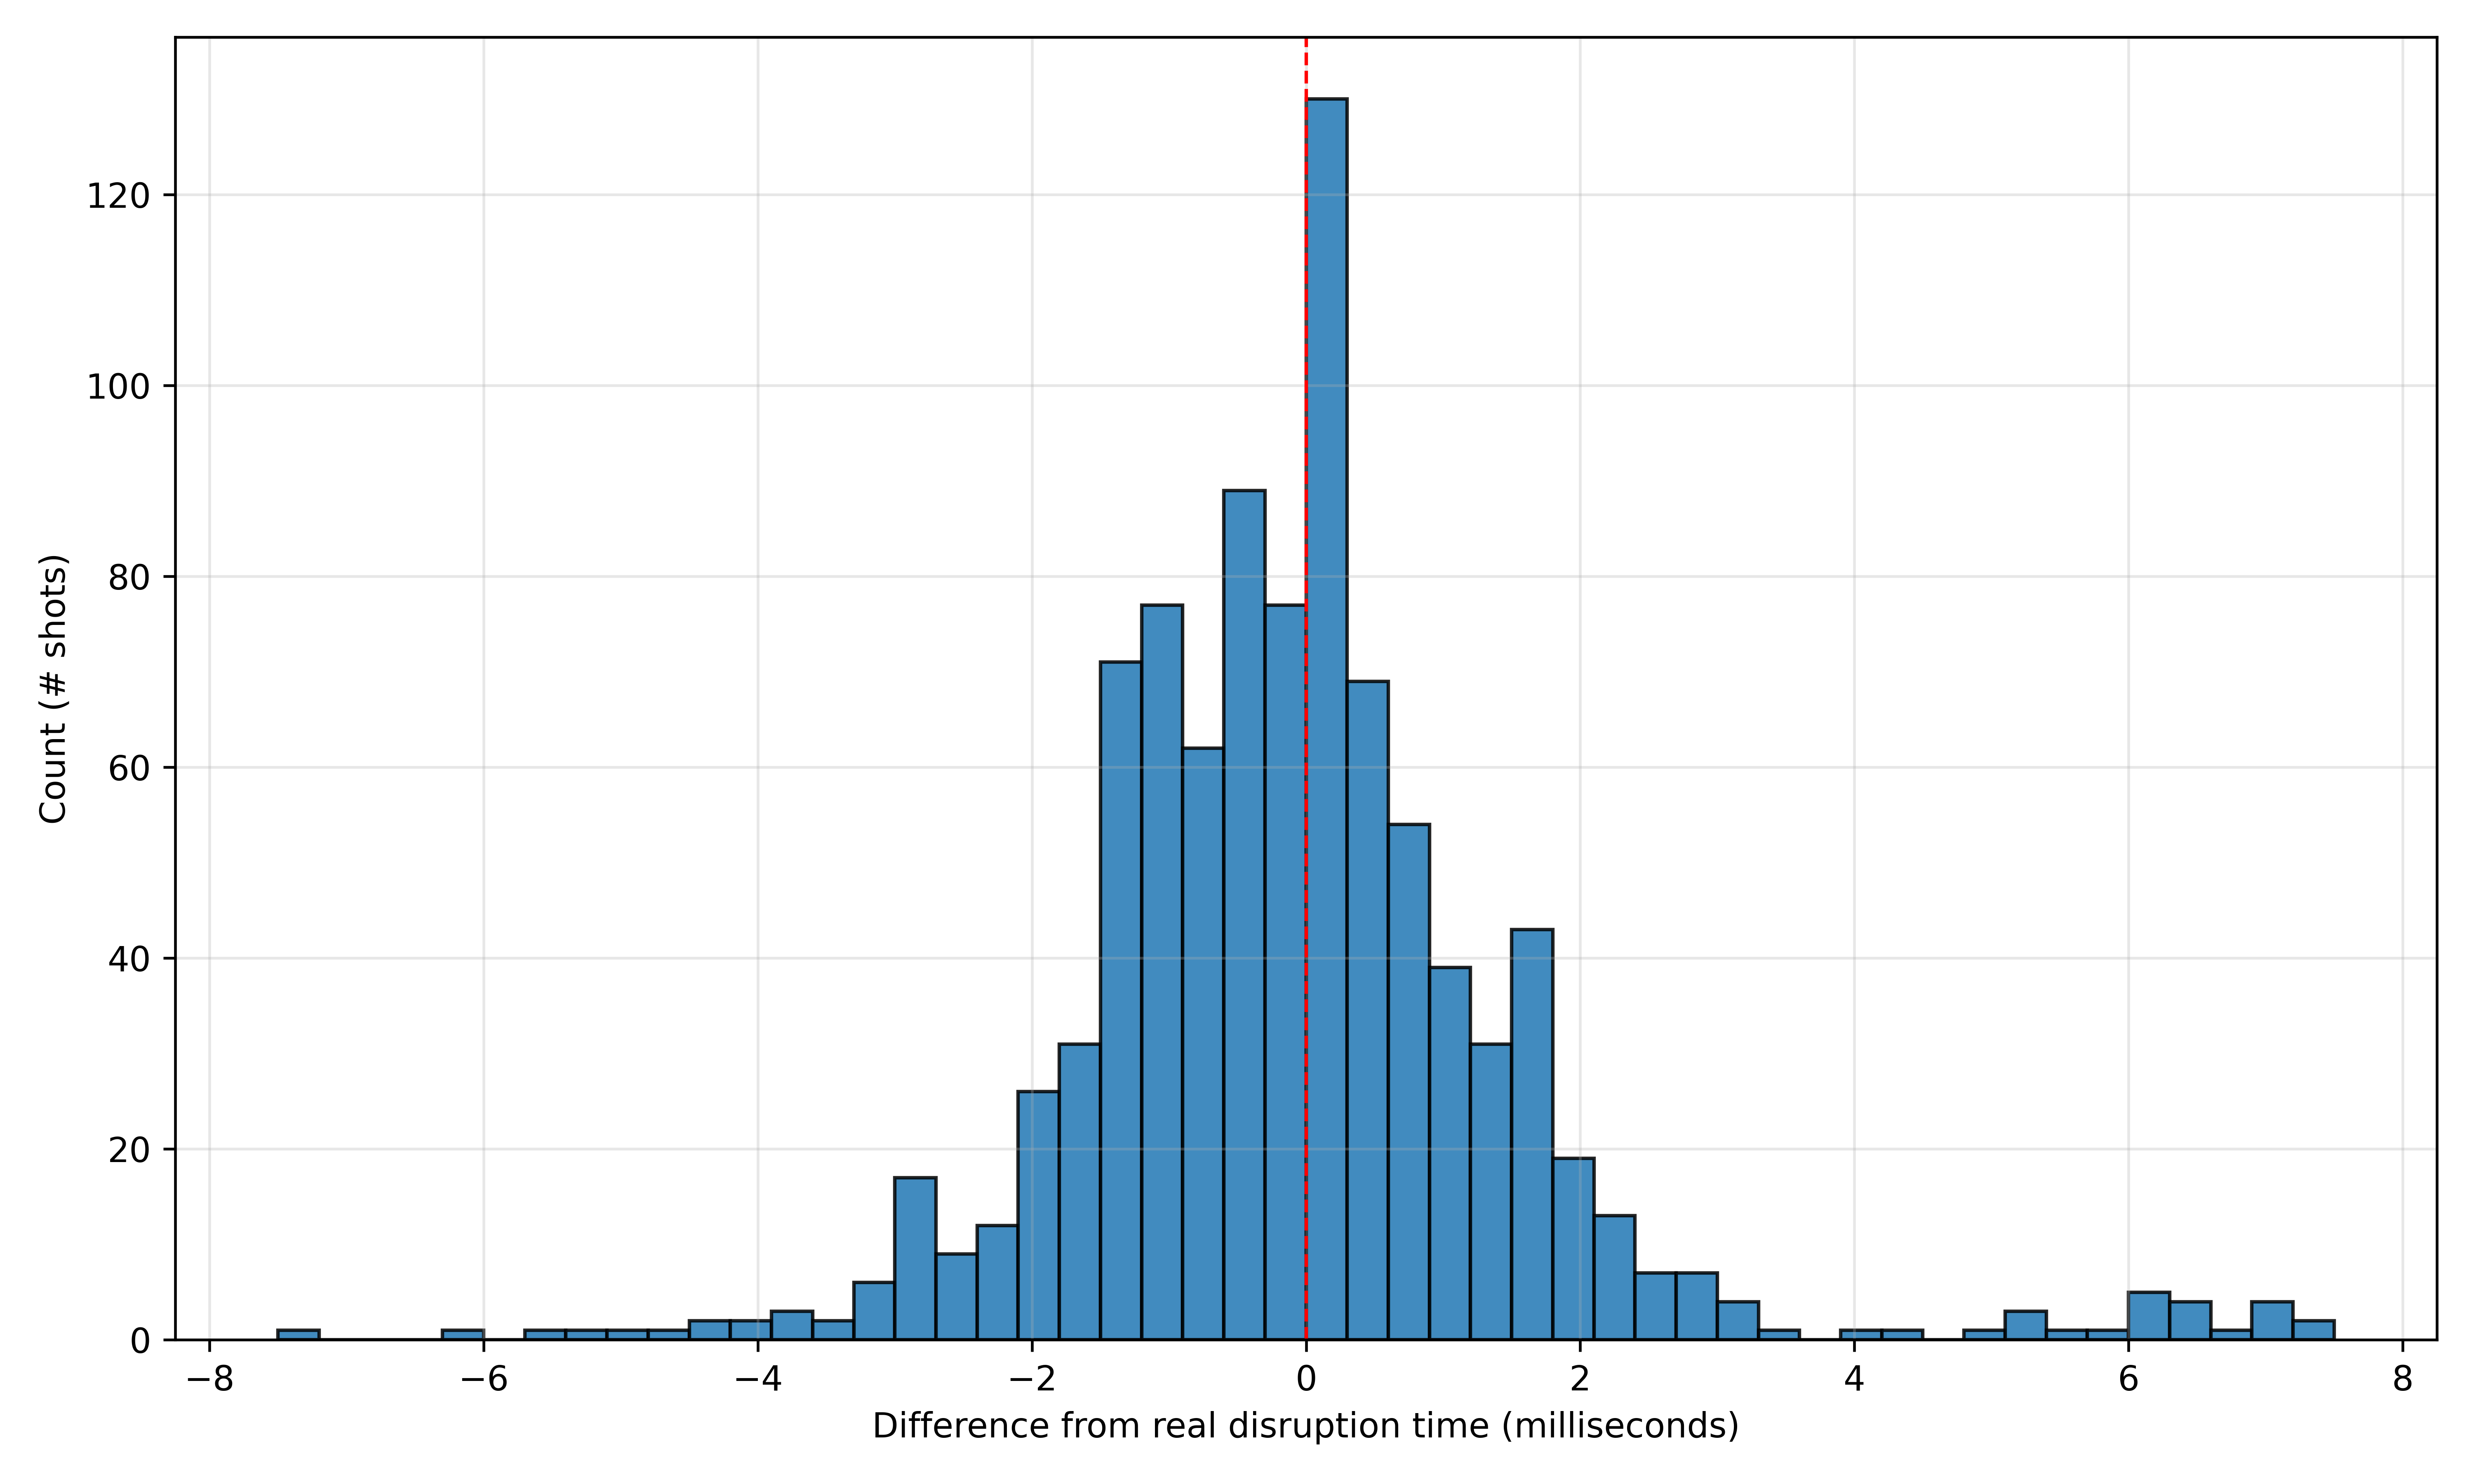
\includegraphics[width=0.8\linewidth]{best_model/disruption_time_diff.png}
  \caption{Figure caption.}
  \label{fig:disruption_time_diff}
\end{figure}



% ==================================================================
\section{Discussion}
\label{sec:discussion}

Interpret results, note limitations, and compare to prior work.

% ==================================================================
\section{Conclusion}
\label{sec:conclusion}

Summarize findings and outline future work.

% ------------------------------------------------------------------
% Optional back matter (uncomment as needed)
% ------------------------------------------------------------------
% \section*{Acknowledgments}
% Funding and thanks.

% \section*{Data and code availability}
% Where artifacts are hosted.

% ------------------------------------------------------------------
\bibliographystyle{unsrtnat}
\bibliography{references}

\end{document}
